\section[Processo de engenharia de requisitos]{Processo de engenharia de requisitos}

A figura \ref{processo} é o modelo proposto baseado no Scalade Agile Framework e nas atividades 5 atividades da engenharia de requisitos: Elicitar; Documentar; Analisar e negociar; Verificar e validar; Gerenciar requisitos. As atividades relacionadas a elicitação então, tratam da especificação em forma de artefato do que o cliente precisa. A documentação é a própria produção dos artefatos. A análise e negociação é a atividade que avalia e negocia o espoco do sistema e sua viabilidade. A verificação e validação é para identificar possíveis inconsistências e incoerências com os requisitos elicitados. O gerenciamento dos requisitos é atividade que acompanha a vida dos requisitos ao longo do desenvolvimento do projeto. Assim, todas essas atividades serão atendidas no modelo proposto.

\begin{figure}[H]
    \centering
    \caption{Processo de requisitos}
    \label{processo}
    \includegraphics[keepaspectratio=true,scale=0.55,angle=90]{figuras/processo.eps}
\end{figure}

\subsection{Papéis do Processo}\label{processoPapeis}
\begin{description}
\item \textbf{Product Owner}

As atividades que o Product Owner (PO) é responsável segundo \cite{leffingwell2011} são:
\begin{itemize}
    \item Trabalhar em harmonia com o Product Manager;
    \item Definir objetivos das sprints;
    \item Manter o backlog da equipe;
    \item Definir prioridades baseados no valor agregado ao usuário;
    \item Elaborar e validar as histórias;
    \item Participar do planejamento e validação da sprint.
\end{itemize}
O papel de PO será desempenhado pelo gestor de pessoas da Zenit Aerospace: Caio

\item \textbf{Product Manager}

O Product Manager (PM) tem as mesmas responsabilidades que o Product Owner, mas com uma diferença é que ele trata a solução por completo. Algumas responsabilidades a mais da do Product Owner são \cite{leffingwell2011}:
\begin{itemize}
    \item Priorizar features;
    \item Manter o Roadmap;
    \item Gerenciar o conteúdo da release;
    \item Priorizar e manter o Backlog do Portfólio;
\end{itemize}

O integrante de requisitos que desempenhará o papel de PM será o Eduardo Nunes da equipe da disciplina de requisitos.

\item \textbf{Scrum master}

O Scrum Master é responsável por garantir que as práticas e regras do Scrum sejam entendidas e aplicadas. Tendo o papel de um servo-líder para a equipe Scrum \cite{agileManifest}. O integrante de requisitos que desempenhará o papel de Scrum Master será o Marcelo Ferreira.

O Scrum Master tem como responsabilidades (1):
\begin{itemize}
    \item Eliminar impedimentos;
    \item Facilitar o progresso da equipe para alcançar a meta;
    \item Reforçar as regras do Scrum sobre a Equipe;
\end{itemize}

\item \textbf{Equipe de Desenvolvimento(time)}

A equipe de desenvolvimento consiste de profissionais que realizam o trabalho de entregar uma versão usável que potencialmente incrementa o produto “Pronto” ao final de cada Sprint (1). Esse papel será desempenhado por todos os integrantes de requisitos.

O papel de Architect/Engineering system, será atribuído ao time, devido o tamanho do projeto e quantidade de membros na equipe de engenharia de requisitos. Esse papel possui a visão geral sobre a arquitetura do sistema e o projeto da solução. Participam das definições de alto nível dos requisitos não funcionais, auxiliam os times a alinharem a visão técnica do desenvolvimento com o documento de visão e roadmap, são responsáveis pela \cite{safe}:
\begin{itemize}
    \item Determinam a tecnologia a ser usada no desenvolvimento do sistema;
    \item Determinação da estrutura geral, componentes e serviços do sistema;
    \item Produzem as histórias habilitadoras;
    \item Critérios de desempenho do sistema como um todo.
\end{itemize}
\end{description}

\subsection{Artefatos}\label{processoArtefatos}

Nessa seção será abordado os artefatos que serão utilizados no sistema analisado, nos três níveis portfólio, programa, e time, segundo o framework SAFe:

\subsubsection{Portfólio}
\begin{itemize}
    \item \textbf{Temas estratégicos:} relacionam os objetivos do negócio do cliente com as estratégias de negócios deles. Fornecem o contexto do negócio para as decisões de investimento no Épicos \cite{safe}.
    \item \textbf{Épicos:} são o segundo nível mais alto de abstração dos requisitos, grandes containes com os valores a serem entregues ao cliente. Este pode conter épicos de negócios e habilitadores. Os épicos habilitadores representam as decisões arquiteturais e os de negócio as funcionalidades \cite{safe}.
    \item \textbf{Backlog de épicos:} artefato para alocar todos os épicos que foram levantados com os clientes e ainda serão produzidos. Assim como contém a prioridade dos épicos que foram aprovados para implementação \cite{safe}.
\end{itemize}

\subsubsection{Programa}
\begin{itemize}
    \item \textbf{Features:} são serviços que tem como propósito suprir alguma necessidade dos stakeholders. Agregam valor para o usuário e são realizadas durante as releases \cite{leffingwell2011}. Existem dois tipos de features no framework adotado, os de negócio, que foi descrito acima, e os enables que são aqueles que descrevem como o sistema irá fazer certa funcionalidade. Ele engloba requisitos de desempenho, de interface externa do sistema, restrições de projeto e atributos da qualidade \cite{safe}.
    \item \textbf{Roadmap do programa:} representa os entregáveis próximos na linha do tempo, ou seja, as features são dispostas em sequência de acordo com a priorização feita. Ele trás visibilidade as features que serão entregues a cada release \cite{safe}.
    \item \textbf{Kanban do programa:} consiste em uma representação visual das features do estado de execução delas como feito, fazendo e a fazer (\textit{done, doing, to do}) \cite{leffingwell2011}.
    \item \textbf{Backlog do programa:} representa um conjunto de features que serão implementadas para o sistema, estas já estão pontuadas de acordo com sua dificuldade técnica \cite{safe}.
    \item \textbf{Visão:} é um conjunto de características que definem quais serão os benefícios que serão entregue para o cliente com a entrega do sistema. Engloba a intenção estratégica do produto, o problema da aplicação, as características e as definições dos requisitos não funcionais \cite{leffingwell2011}. 
\end{itemize}
\subsubsection{Time}
\begin{itemize}
    \item \textbf{Histórias:} breve descrição de uma funcionalidade que foi discutida \cite{leffingwell2011}. Histórias de usuário não são requisitos e sim pequenas pedaços da funcionalidade de um software descritos na linguagem natural de um usuário \cite{safe}. Neste framework, as histórias são tratadas como de usuário e enables.
    \item \textbf{Backlog de história:} representa conjunto de histórias priorizadas de acordo com os interesses do cliente e restrições entre histórias, que serão implementadas para o sistema durante uma sprint \cite{safe}.
    \item \textbf{Historias pontuadas:} são histórias com a pontuação referente ao nível de dificuldade, complexidade e esforço para sua implementação.
    \item \textbf{Resumo retrospectiva:} é um resumo de todos os tópicos discutidos na retrospectiva da sprint. Serve para avaliar a forma que que tem que ser melhorado para a próxima sprint.
    \item \textbf{Kanban de time:} consiste em uma representação visual das histórias de usuários que estão realizadas, as que estão sendo realizadas e as que não começaram a ser realizadas \cite{leffingwell2011}.
    \item \textbf{Atividade e seus artefatos envolvidos:} nessa seção será abordado os artefatos que serão utilizados no sistema nos três níveis portfólio, programa, e time, analisando os artefatos que precisam ser gerados, citados na seção anterior.
\end{itemize}

\subsection{Descrição de tividades}

As descrições das atividades de cada subprocesso a seguir contém as informações de acordo com o quadro \ref{descricaoAtividades}. Essas informações são as necessárias para que a equipe de elicitação seja capaz de desempenhar cada aditividade corretamente.

\begin{table}[H]
    \centering
    \label{descricaoAtividades}
    \caption{Formato de descrição das atividades}
        \begin{tabular}{|l|p{10cm}|}
        \hline
        \textbf{Nome} & Nome significativo, coerente com a descrição da atividade \\
        \hline
        \textbf{Artefato(s) de entrada} & Indica quais são os artefatos \ref{processoArtefatos} já produzidos que serão necessários para o desenvolvimento desta atividade \\
        \hline
        \textbf{Descrição} & Descreve resumidamente quais serão os passos necessários para que a atividade seja executada, e possibilite a sua execução. \\
        \hline
        \textbf{Artefato de saída} & Após a execução da atividade, os artefatos \ref{processoArtefatos} produzidos são listados neste campo. \\
        \hline
        \textbf{Responsável} & Dentre os papeis descritos \ref{processoPapeis}, aqui será indicado qual o papel responsável pela execução da tarefa.\\
        \hline
    \end{tabular}
\end{table}

\subsubsection{Portfólio}

Neste nível do SAFe, os requisitos são tratados de forma mais abstrata e menos detalhada. Identifica-se as necessidades e o problema da empresa. Assim como os interesses de investimentos dela, representados pelos temas estratégicos.
\begin{enumerate}
\item \textbf{Subprocesso identificar interesses da empresa}

Este sub processo, imagem \ref{processoInteresses} representa um conjunto de atividades voltadas ao levantamento dos interesses de investimento do cliente para sua empresa. Define-se os temas estratégicos da empresa.

\begin{figure}[H]
    \centering
    \caption{Identificar interesses da empresa}
    \label{processoInteresses}
    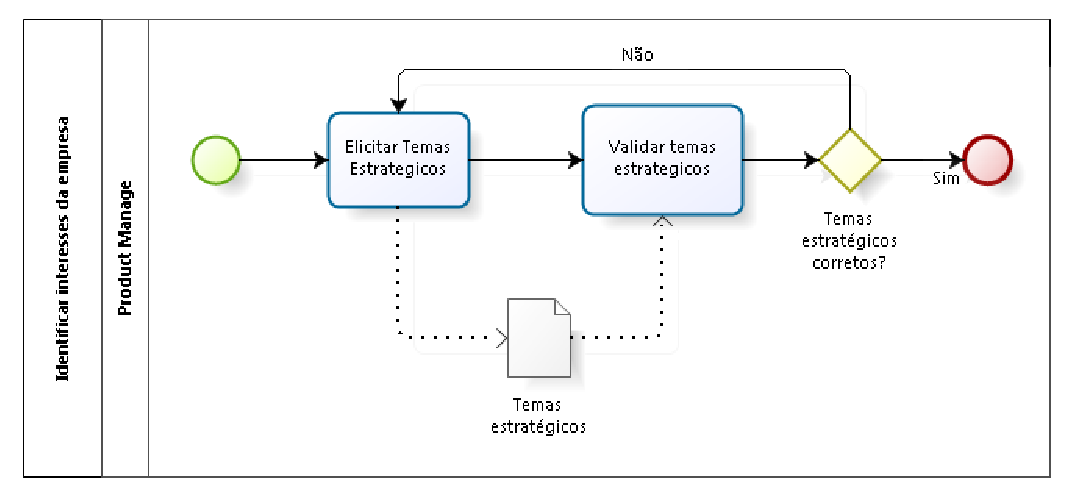
\includegraphics[keepaspectratio=true,scale=0.6]{figuras/processoInteresses.eps}
\end{figure}

\begin{table}[H]
    \centering
    \label{descricaoAtividades1}
    \caption{Descrição da atividade elicitar temas estratégicos}
        \begin{tabular}{|l|p{10cm}|}
        \hline
        \textbf{Nome} & Elicitar temas estratégicos \\
        \hline
        \textbf{Artefato(s) de entrada} & Contexto do negócio \\
        \hline
        \textbf{Descrição} & Reunião com o cliente utilizando técnicas de elicitação de requisitos para identificar as oportunidades de negócio. \\
        \hline
        \textbf{Artefato de saída} & Temas estratégicos elicitados \\
        \hline
        \textbf{Responsável} & Product manager\\
        \hline
    \end{tabular}
\end{table}

\begin{table}[H]
    \centering
    \label{descricaoAtividades2}
    \caption{Descrição da atividade validar temas estratégicos}
        \begin{tabular}{|l|p{10cm}|}
        \hline
        \textbf{Nome} & Validar temas estratégicos \\
        \hline
        \textbf{Artefato(s) de entrada} & Temas estratégicos \\
        \hline
        \textbf{Descrição} & Validar com o cliente se os temas estratégicos correspondem aos interesses de investimento da empresa naquele momento \\
        \hline
        \textbf{Artefato de saída} & Temas estratégicos validados \\
        \hline
        \textbf{Responsável} & Product manager\\
        \hline
    \end{tabular}
\end{table}

\item \textbf{Subprocesso identificar valores para empresa}
\end{enumerate}
O produto a ser desenvolvido, em um nível mais abstrato, define quais os valores que esse entregará ao cliente, empresa. Assim sendo, este subprocesso trata de identificar e priorizar os itens que proverão valores a empresa, representados pelos artefatos épicos.

\begin{figure}[H]
    \centering
    \caption{Identificar valores da empresa}
    \label{processoValores}
    \includegraphics[keepaspectratio=true,scale=0.4]{figuras/processoValores.eps}
\end{figure}

\begin{table}[H]
    \centering
    \label{descricaoAtividades3}
    \caption{Descrição da atividade elicitar épicos} 
        \begin{tabular}{|l|p{10cm}|}
        \hline
        \textbf{Nome} & Elicitar épicos \\
        \hline
        \textbf{Artefato(s) de entrada} & Temas estratégicos \\
        \hline
        \textbf{Descrição} & Reunião com o cliente utilizando técnicas de elicitação de requisitos para identificar os épicos de negócios e habilitadores. \\
        \hline
        \textbf{Artefato de saída} & Épicos \\
        \hline
        \textbf{Responsável} & Product manager \\
        \hline
    \end{tabular}
\end{table}

\begin{table}[H]
    \centering
    \label{descricaoAtividades4}
    \caption{Descrição da atividade analisar viabilidade de épicos}
        \begin{tabular}{|l|p{10cm}|}
        \hline
        \textbf{Nome} & Analisar viabilidade de épicos \\
        \hline
        \textbf{Artefato(s) de entrada} & Épicos \\
        \hline
        \textbf{Descrição} & Determinar se os épicos, tanto de negócio quanto habilitadores, são viáveis com base na tecnologia, tempo e custo. Se necessário dividir em mais épicos. \\
        \hline
        \textbf{Artefato de saída} & Épicos analisados \\
        \hline
        \textbf{Responsável} & Product manager \\
        \hline
    \end{tabular}
\end{table}

\begin{table}[H]
    \centering
    \label{descricaoAtividades5}
    \caption{Descrição da atividade verificar e validar épicos}
        \begin{tabular}{|l|p{10cm}|}
        \hline
        \textbf{Nome} & Verificar e validar épicos \\
        \hline
        \textbf{Artefato(s) de entrada} & Épicos analisados \\
        \hline
        \textbf{Descrição} & Verificar com o cliente se os épicos analisados correspondem aos itens que o cliente deseja. \\
        \hline
        \textbf{Artefato de saída} & Épicos verificados e validados. \\
        \hline
        \textbf{Responsável} & Product Owner \\
            \hline
        \end{tabular}
    \end{table}

    \begin{table}[H]
        \centering
        \label{descricaoAtividades6}
        \caption{Descrição da atividade criar backlog de épicos}
            \begin{tabular}{|l|p{10cm}|}
            \hline
            \textbf{Nome} & Criar backlog de épicos \\
            \hline
            \textbf{Artefato(s) de entrada} & Épicos verificados e validados \\
            \hline
            \textbf{Descrição} & Criar o backlog com os épicos de acordo com as priorizações estabelecidas pela atividade de priorizar épicos. \\
            \hline
            \textbf{Artefato de saída} & Backlog de épicos. \\
            \hline
            \textbf{Responsável} & Product owner \\
            \hline
        \end{tabular}
    \end{table}

    \begin{table}[H]
        \centering
        \label{descricaoAtividades7}
        \caption{Descrição da atividade priorizar épicos}
            \begin{tabular}{|l|p{10cm}|}
            \hline
            \textbf{Nome} & Priorizar épicos \\
            \hline
            \textbf{Artefato(s) de entrada} & Backlog de épicos \\
            \hline
            \textbf{Descrição} & Reunir e classificar os épicos de acordo com sua importância para os interesses de negócio do cliente. Assim como definir as relações de dependência entre eles. \\
            \hline
            \textbf{Artefato de saída} & Épicos priorizados. \\
            \hline
            \textbf{Responsável} & Product owner \\
            \hline
        \end{tabular}
    \end{table}

    \subsubsection{Programa}
    \begin{enumerate}
    \item \textbf{Subprocesso desenvolver programa}
    \end{enumerate}
    O nível de programa é o onde as features são definidas, avaliadas e documentadas. O conjunto de atividades a seguir permitem que sejam elaborado o conjunto de features que representam as várias características do produto final de acordo com um épico a ser entregue para o cliente.

    \begin{figure}[H]
        \centering
        \caption{Desenvolver programa}
        \label{processoPrograma}
        \includegraphics[keepaspectratio=true,scale=0.3]{figuras/processoPrograma.eps}
    \end{figure}

    \begin{table}[H]
        \centering
        \label{descricaoAtividades8}
        \caption{Descrição da atividade elicitar features}
            \begin{tabular}{|l|p{10cm}|}
            \hline
            \textbf{Nome} & Elicitar features \\
            \hline
            \textbf{Artefato(s) de entrada} & Épico priorizados. \\
            \hline
            \textbf{Descrição} & Essa atividade é responsável pelo levantamento das features de negócio e habilitadores que serão necessárias para realização de cada release. \\
            \hline
            \textbf{Artefato de saída} & Features \\
            \hline
            \textbf{Responsável} & Product manager \\
            \hline
        \end{tabular}
    \end{table}

    \begin{table}[H]
        \centering
        \label{descricaoAtividades9}
        \caption{Descrição da atividade analisar features}
            \begin{tabular}{|l|p{10cm}|}
            \hline
            \textbf{Nome} & Analisar features \\
            \hline
            \textbf{Artefato(s) de entrada} & Features \\
            \hline
            \textbf{Descrição} & Analisar as features elaboradas, e estimar o escopo das features determinar sua viabilidade técnica e averiguar a possibilidade de dividir em itens menores para o backlog. \\
            \hline
            \textbf{Artefato de saída} & Features analisadas \\
            \hline
            \textbf{Responsável} & Product manager \\
            \hline
        \end{tabular}
    \end{table}

    \begin{table}[H]
        \centering
        \label{descricaoAtividades10}
        \caption{Descrição da atividade verificar e validar features}
            \begin{tabular}{|l|p{10cm}|}
            \hline
            \textbf{Nome} & Verificar e validar features \\
            \hline
            \textbf{Artefato(s) de entrada} & Features analisadas \\
            \hline
            \textbf{Descrição} & Verificar e validar com o Product onwer as features que foram analisadas se elas correspondem as necessidades do cliente, empresa. \\
            \hline
            \textbf{Artefato de saída} & Features validadas \\
            \hline
            \textbf{Responsável} & Product Manager \\
            \hline
        \end{tabular}
    \end{table}

    \begin{table}[H]
        \centering
        \label{descricaoAtividades11}
        \caption{Descrição da atividade montar backlog de features}
            \begin{tabular}{|l|p{10cm}|}
            \hline
            \textbf{Nome} & Montar backlog de features \\
            \hline
            \textbf{Artefato(s) de entrada} & Features validadas. \\
            \hline
            \textbf{Descrição} & Agrupar todas as features validadas com o cliente que ainda não foram implementadas em um único documento, a fim de se ter visão do que será produzido para o produto. \\
            \hline
            \textbf{Artefato de saída} & Backlog de features. \\
            \hline
            \textbf{Responsável} & Product manager \\
            \hline
        \end{tabular}
    \end{table}

    \begin{table}[H]
        \centering
        \label{descricaoAtividades12}
        \caption{Descrição da atividade priorizar features}
            \begin{tabular}{|l|p{10cm}|}
            \hline
            \textbf{Nome} & Priorizar features \\
            \hline
            \textbf{Artefato(s) de entrada} & Backlog de features; \\
            \hline
            \textbf{Descrição} & Classificar as features de acordo com sua importância para o projeto, ou seja, classifica-se pelo valor entregue, redução de risco, oportunidade de habilitar um valor. \\
            \hline
            \textbf{Artefato de saída} & Roadmap de features. \\
            \hline
            \textbf{Responsável} & Product manager \\
            \hline
        \end{tabular}
    \end{table}

    \begin{table}[H]
        \centering
        \label{descricaoAtividades13}
        \caption{Descrição da atividade elaborar visão}
            \begin{tabular}{|l|p{10cm}|}
            \hline
            \textbf{Nome} & Elaborar visão \\
            \hline
            \textbf{Artefato(s) de entrada} & Roadmap de features. \\
            \hline
            \textbf{Descrição} & Escreve o documento de visão do projeto com as decisões tomadas na etapa de desenvolver do programa. \\
            \hline
            \textbf{Artefato de saída} & Documento de visão. \\
            \hline
            \textbf{Responsável} & Product manager \\
            \hline
        \end{tabular}
    \end{table}

    \begin{table}[H]
        \centering
        \label{descricaoAtividades14}
        \caption{Descrição da atividade elaborar kanban de features}
            \begin{tabular}{|l|p{10cm}|}
            \hline
            \textbf{Nome} & Elaborar Kanban de features \\
            \hline
            \textbf{Artefato(s) de entrada} & Roadmap de features. \\
            \hline
            \textbf{Descrição} & Elabora o Kaban de features com as decisões tomadas na etapa de desenvolver do programa. \\
            \hline
            \textbf{Artefato de saída} & Kanban de features. \\
            \hline
            \textbf{Responsável} & Product manager \\
            \hline
        \end{tabular}
    \end{table}

    \subsubsection{Time}
    \begin{enumerate}
    \item \textbf{ Subprocesso identificar histórias}

    Nesta etapa do processo, as features definidas serão detalhadas na forma de histórias de usuário elicitados com os usuários. A fim de prover um conjunto de histórias priorizadas para a implementação.

    \begin{figure}[H]
        \centering
        \caption{Identificar histórias}
        \label{processoHistorias}
        \includegraphics[keepaspectratio=true,scale=0.5]{figuras/processoHistorias.eps}
    \end{figure}

    \begin{table}[H]
        \centering
        \label{descricaoAtividades15}
        \caption{Descrição da atividade elicitar histórias}
            \begin{tabular}{|l|p{10cm}|}
            \hline
            \textbf{Nome} & Elicitar histórias \\
            \hline
            \textbf{Artefato(s) de entrada} & Kanban de features e o Documento de visão. \\
            \hline
            \textbf{Descrição} & Consiste no levantamento das histórias feitas pelo time juntamente com o product owner, utilizando as técnicas de elicitações. Os tipos de histórias elicitados serão histórias de usuário e habilitadoras. \\
            \hline
            \textbf{Artefato de saída} & Histórias elicitadas. \\
            \hline
            \textbf{Responsável} & Time \\
            \hline
        \end{tabular}
    \end{table}

    \begin{table}[H]
        \centering
        \label{descricaoAtividades16}
        \caption{Descrição da atividade definir critério de aceitação}
            \begin{tabular}{|l|p{10cm}|}
            \hline
            \textbf{Nome} & Definir critério de aceitação \\
            \hline
            \textbf{Artefato(s) de entrada} & Historias elicitadas. \\
            \hline
            \textbf{Descrição} & Consiste em definir quais são os critérios que devem ser seguidos para que a histórias de usuário sejam aceitas como completadas. \\
            \hline
            \textbf{Artefato de saída} & Historias de usuário com critérios de aceitação. \\
            \hline
            \textbf{Responsável} & Time \\
            \hline
        \end{tabular}
    \end{table}

    \begin{table}[H]
        \centering
        \label{descricaoAtividades17}
        \caption{Descrição da atividade elicitar histórias}
            \begin{tabular}{|l|p{10cm}|}
            \hline
            \textbf{Nome} & Elicitar histórias \\
            \hline
            \textbf{Artefato(s) de entrada} & Kanban de features e o Documento de visão. \\
            \hline
            \textbf{Descrição} & Consiste no levantamento das histórias feitas pelo time juntamente com o product owner, utilizando as técnicas de elicitações. Os tipos de histórias elicitados serão histórias de usuário e habilitadoras. \\
            \hline
            \textbf{Artefato de saída} & Histórias elicitadas. \\
            \hline
            \textbf{Responsável} & Time \\
            \hline
        \end{tabular}
    \end{table}

    \begin{table}[H]
        \centering
        \label{descricaoAtividades18}
        \caption{Descrição da atividade priorizar histórias}
            \begin{tabular}{|l|p{10cm}|}
            \hline
            \textbf{Nome} & Priorizar histórias \\
            \hline
            \textbf{Artefato(s) de entrada} & Backlog de histórias. \\
            \hline
            \textbf{Descrição} & As histórias de usuário serão priorizadas de acordo com a complexidade, esforço necessário, recursos humanos para a realização das atividades. \\
            \hline
            \textbf{Artefato de saída} & Backlog priorizado. \\
            \hline
            \textbf{Responsável} & Product Owner \\
            \hline
        \end{tabular}
    \end{table}

    \item \textbf{Subprocesso Planejar sprint}

    Nessa seção serão definidas as atividades necessárias para projetar uma sprint.
    \begin{figure}[H]
        \centering
        \caption{Planejar sprint}
        \label{processoPlanejar}
        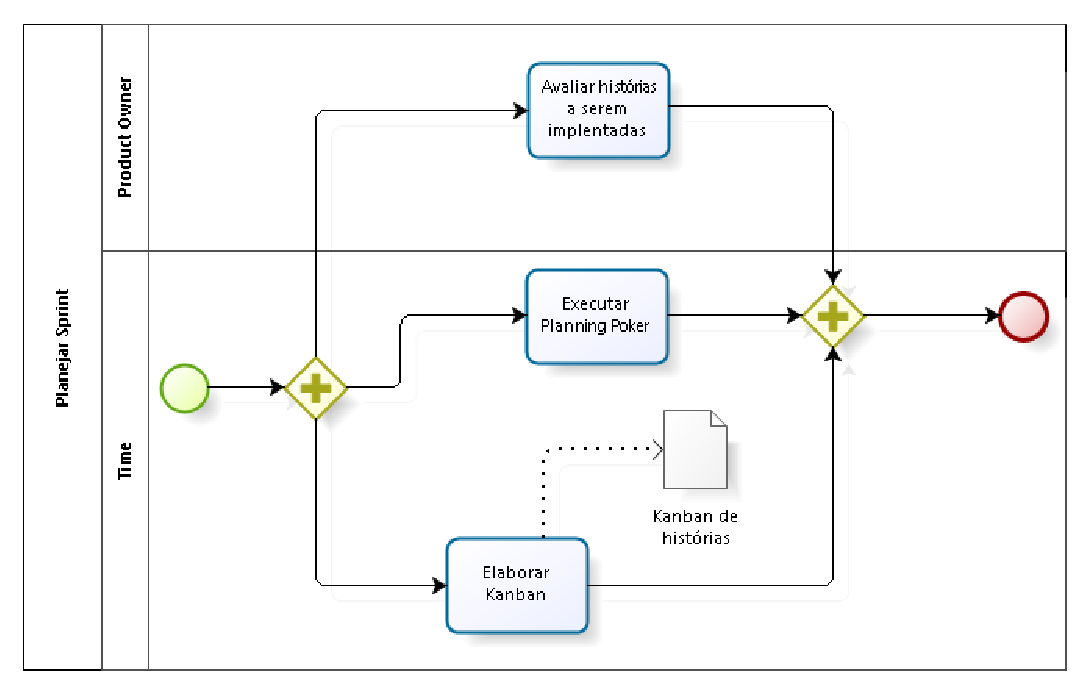
\includegraphics[keepaspectratio=true,scale=0.5]{figuras/processoPlanejar.eps}
    \end{figure}

    \begin{table}[H]
        \centering
        \label{descricaoAtividades19}
        \caption{Descrição da atividade avaliar histórias a serem implementadas}
            \begin{tabular}{|l|p{10cm}|}
            \hline
            \textbf{Nome} & Avaliar histórias a serem implementadas \\
            \hline
            \textbf{Artefato(s) de entrada} & Backlog priorizado. \\
            \hline
            \textbf{Descrição} & Nesta atividade, o time e o Product Owner decidirão quais as histórias que serão implementadas durante a sprint. Essa atividade será realizada em paralelo com a atividade “planning poker”. \\
            \hline
            \textbf{Artefato de saída} & Kanban de histórias. \\
            \hline
            \textbf{Responsável} & Time \\
            \hline
        \end{tabular}
    \end{table}

    \begin{table}[H]
        \centering
        \label{descricaoAtividades20}
        \caption{Descrição da atividade executar planning poker}
            \begin{tabular}{|l|p{10cm}|}
            \hline
            \textbf{Nome} & Executar planning poker \\
            \hline
            \textbf{Artefato(s) de entrada} & Backlog priorizado. \\
            \hline
            \textbf{Descrição} & Essa atividade descreve a pontuação em forma de um “jogo de poker” em que o time pontua a história de acordo com o nível de dificuldade para implementá-la. Essa pontuação só tem números da sequência de Fibonacci. \\
            \hline
            \textbf{Artefato de saída} & Kanban de histórias. \\
            \hline
            \textbf{Responsável} & Time \\
            \hline
        \end{tabular}
    \end{table}

    \begin{table}[H]
        \centering
        \label{descricaoAtividades20}
        \caption{Descrição da atividade elaborar kanban}
            \begin{tabular}{|l|p{10cm}|}
            \hline
            \textbf{Nome} & Elaborar kanban \\
            \hline
            \textbf{Artefato(s) de entrada} & Backlog priorizado \\
            \hline
            \textbf{Descrição} & Definir quais são as histórias de usuário que serão utilizadas no backlog de histórias para serem implementadas na sprint. \\
            \hline
            \textbf{Artefato de saída} & Kanban de histórias. \\
            \hline
            \textbf{Responsável} & Time \\
            \hline
        \end{tabular}
    \end{table}

    \item \textbf{Executar Sprint}
    \end{enumerate}
    Nessa seção será definida as atividades necessárias durante a realização de uma sprint.

    \begin{figure}[H]
        \centering
        \caption{Executar sprint}
        \label{processoExecutar}
        \includegraphics[keepaspectratio=true,scale=0.5]{figuras/processoExecutar.eps}
    \end{figure}

    \begin{table}[H]
        \centering
        \label{descricaoAtividades21}
        \caption{Descrição da atividade desenvolver histórias}
            \begin{tabular}{|l|p{10cm}|}
            \hline
            \textbf{Nome} & Desenvolver histórias \\
            \hline
            \textbf{Artefato(s) de entrada} & História de usuário \\
            \hline
            \textbf{Descrição} & Consiste na implementação das funcionalidades, requisitos não funcionais, ou seja, produzir o software pela definição na história de usuário ou habilitadora. \\
            \hline
            \textbf{Artefato de saída} & Código fonte \\
            \hline
            \textbf{Responsável} & Time \\
            \hline
        \end{tabular}
    \end{table}

    \begin{table}[H]
        \centering
        \label{descricaoAtividades22}
        \caption{Descrição da atividade fazer retrospectiva e revisão}
            \begin{tabular}{|l|p{10cm}|}
            \hline
            \textbf{Nome} & Fazer retrospectiva e revisão \\
            \hline
            \textbf{Artefato(s) de entrada} & Gráfico burndown. \\
            \hline
            \textbf{Descrição} & Consiste em analisar a qualidade do trabalho feito, definindo pontos bons e ruins da equipe. \\
            \hline
            \textbf{Artefato de saída} & Resumo retrospectiva. \\
            \hline
            \textbf{Responsável} & Time \\
            \hline
        \end{tabular}
    \end{table}

    \begin{table}[H]
        \centering
        \label{descricaoAtividades23}
        \caption{Descrição da atividade desenhar burndown}
            \begin{tabular}{|l|p{10cm}|}
            \hline
            \textbf{Nome} & Desenhar burndown \\
            \hline
            \textbf{Artefato(s) de entrada} & Kanban de histórias. \\
            \hline
            \textbf{Descrição} & Consiste em gerar um gráfico com os pontos executados durante uma sprint. \\
            \hline
            \textbf{Artefato de saída} & Gráfico burndown. \\
            \hline
            \textbf{Responsável} & Scrum Master \\
            \hline
        \end{tabular}
    \end{table}

    \subsubsection{Subprocesso Gerência de Requisitos}


    A engenharia de requisitos é um processo que engloba todas as atividades que contribuem para a produção de um documento de requisitos e sua manutenção ao longo do tempo.

    Como a equipe de desenvolvimento de requisitos é pequena, todos os envolvidos participarão em todos os níveis: Temas estratégicos, Épicos, Features e Histórias. Não há necessidade de definir um subprocesso de gerência para cada um dos níveis, apesar de haver distinção no tratamento da gerência de requisitos em cada um deles, pois mudanças nos épicos, influenciarão features e histórias de usuário, enquanto que mudanças nas histórias influenciarão principalmente outras histórias. Ainda assim, as atividades descritas neste subprocesso são capazes de atingir as necessidades de gestão em cada um dos três níveis.

    \begin{figure}[H]
        \centering
        \caption{Gerencia de requisitos}
        \label{processoGerencia}
        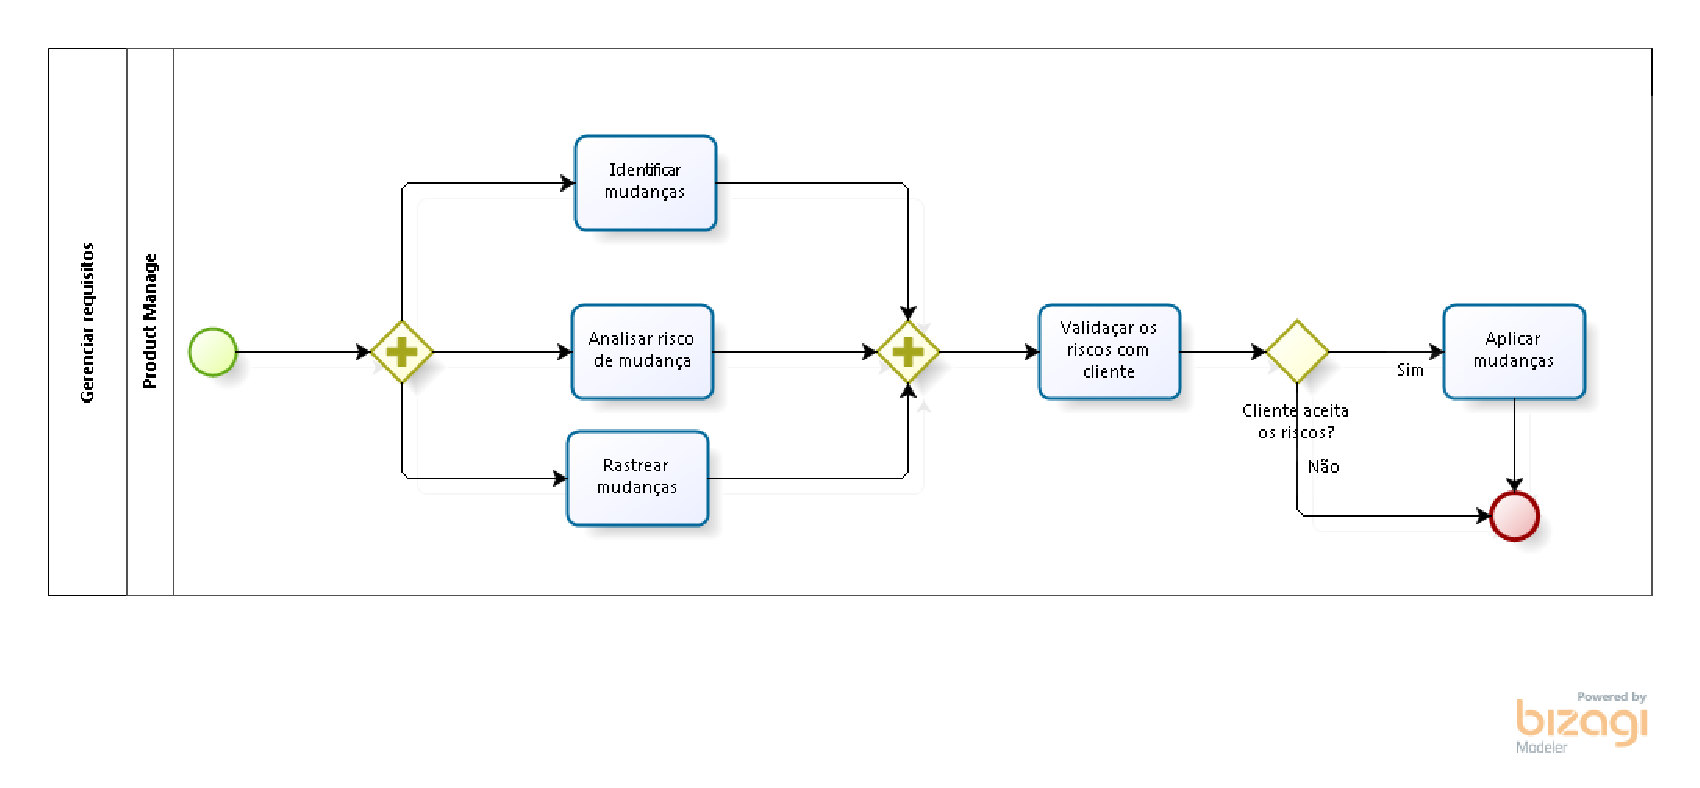
\includegraphics[keepaspectratio=true,scale=0.5]{figuras/processoGerencia.eps}
    \end{figure}

    \begin{table}[H]
        \centering
        \label{descricaoAtividades24}
        \caption{Descrição da atividade identificar mudanças}
            \begin{tabular}{|l|p{10cm}|}
            \hline
            \textbf{Nome} & Identificar mudanças \\
            \hline
            \textbf{Artefato(s) de entrada} & Não validação dos artefatos. \\
            \hline
            \textbf{Descrição} & Essa atividade é responsável por identificar as mudanças necessárias quando algum artefato não foi validado. \\
            \hline
            \textbf{Artefato de saída} & Documento de mudança. \\
            \hline
            \textbf{Responsável} & Product manager \\
            \hline
        \end{tabular}
    \end{table}

    \begin{table}[H]
        \centering
        \label{descricaoAtividades25}
        \caption{Descrição da atividade rastrear mudanças}
            \begin{tabular}{|l|p{10cm}|}
            \hline
            \textbf{Nome} & Rastrear mudanças \\
            \hline
            \textbf{Artefato(s) de entrada} & Documento de mudança. \\
            \hline
            \textbf{Descrição} & Essa atividade é responsável por identificar onde as mudanças serão aplicadas e caso se a mudança vier de um nível anterior, mandar essa análise para a gerência do nível necessário. \\
            \hline
            \textbf{Artefato de saída} & Documento de mudança rastreado. \\
            \hline
            \textbf{Responsável} & Product manager \\
            \hline
        \end{tabular}
    \end{table}

    \begin{table}[H]
        \centering
        \label{descricaoAtividades26}
        \caption{Descrição da atividade analisar risco da mudança}
            \begin{tabular}{|l|p{10cm}|}
            \hline
            \textbf{Nome} & Analisar risco da mudança \\
            \hline
            \textbf{Artefato(s) de entrada} & Documento de mudança rastreado. \\
            \hline
            \textbf{Descrição} & Essa atividade é responsável por analisar os impactos das mudanças para que seja possível saber se as mudanças são ou não viáveis. \\
            \hline
            \textbf{Artefato de saída} & Documento de mudança com riscos. \\
            \hline
            \textbf{Responsável} & Product manager \\
            \hline
        \end{tabular}
    \end{table}

    \begin{table}[H]
        \centering
        \label{descricaoAtividades27}
        \caption{Descrição da atividade validar os riscos com cliente}
            \begin{tabular}{|l|p{10cm}|}
            \hline
            \textbf{Nome} & Validar os riscos com cliente \\
            \hline
            \textbf{Artefato(s) de entrada} & Documento de mudança com riscos. \\
            \hline
            \textbf{Descrição} & Essa atividade será realizada com o Product Owner para que ele possa validar as mudanças levando em consideração os riscos das mudanças e definir se serão implantadas. \\
            \hline
            \textbf{Artefato de saída} & Documento de mudança validado. \\
            \hline
            \textbf{Responsável} & Product manager \\
            \hline
        \end{tabular}
    \end{table}

    \begin{table}[H]
        \centering
        \label{descricaoAtividades28}
    \caption{Descrição da atividade aplicar mudanças}
        \begin{tabular}{|l|p{10cm}|}
        \hline
        \textbf{Nome} & Aplicar mudanças \\
        \hline
        \textbf{Artefato(s) de entrada} & Documento de mudança validado. \\
        \hline
        \textbf{Descrição} & Caso se as mudanças apresentarem um benefício maior do que o risco, essa atividade será responsável por aplicá-las em seus devidos lugares. \\
        \hline
        \textbf{Artefato de saída} & Mudanças realizadas. \\
        \hline
        \textbf{Responsável} & Product manager \\
        \hline
    \end{tabular}
\end{table}


